% options:
% hidelinks remove colour boxes around hyperlinks
\documentclass[thesis=B,czech]{FITthesis}[2012/06/26]

\usepackage[utf8]{inputenc} % LaTeX source encoded as UTF-8
\usepackage{graphicx} %graphics files inclusion
% \usepackage{amsmath} %advanced maths
% \usepackage{amssymb} %additional math symbols
\usepackage{dirtree} %directory tree visualisation

\usepackage{listings}


% % list of acronyms
% \usepackage[acronym,nonumberlist,toc,numberedsection=autolabel]{glossaries}
% \iflanguage{czech}{\renewcommand*{\acronymname}{Seznam pou{\v z}it{\' y}ch zkratek}}{}
% \makeglossaries

\newcommand{\tg}{\mathop{\mathrm{tg}}} %cesky tangens
\newcommand{\cotg}{\mathop{\mathrm{cotg}}} %cesky cotangens

\department{Katedra softwarového inženýrství}
\title{Flexibilní logování pro embedded Linuxové systémy}
\authorGN{David} %(křestní) jméno (jména) autora
\authorFN{Vavřička} %příjmení autora
\authorWithDegrees{David Vavřička} %jméno autora včetně současných akademických titulů
\supervisor{Ing. Matěj Laitl}
\acknowledgements{Doplňte, máte-li komu a za co děkovat. V~opačném případě úplně odstraňte tento příkaz.}
\abstractCS{Doplňte}
\abstractEN{Sem doplňte ekvivalent abstraktu Vaší práce v~angličtině.}
\placeForDeclarationOfAuthenticity{V~Praze}
\declarationOfAuthenticityOption{4} %volba Prohlášení (číslo 1-6)
\keywordsCS{logování, vestavěné systémy, logovací démoni, Linux, Rsyslog}
\keywordsEN{logging, embedded systems, logging daemons, Linux, Rsyslog}

\begin{document}

% \newacronym{CVUT}{{\v C}VUT}{{\v C}esk{\' e} vysok{\' e} u{\v c}en{\' i} technick{\' e} v Praze}
% \newacronym{FIT}{FIT}{Fakulta informa{\v c}n{\' i}ch technologi{\' i}}

\begin{introduction}

\end{introduction}

\chapter{Technické požadavky}
Cílem je upravit logovací řešení pro set-top box EKT DID7006mTF~\cite{ekt7006} tak, aby splňovalo technické požadavky popsané v této kapitole. Řešení musí fungovat a být otestováno na zmíněném modelu set-top boxu a pokud možno by mělo být přenositelné i na jiné typy set-top boxů.
Požadavky jsou rozděleny na základní a rozšířené. Rozšířené požadavky není nutno implementovat.

\section{Základní technické požadavky}

\subsection{Snížení objemu logů}
Je žádoucí umožnit snížit objem zasílaných logů z důvodu přílišného zatížení sítě a serverových disků. A to tak, že zadavatel bude schopen nadefinovat pro každou komponentu úroveň severity zpráv, od které mají být posílány na server. Výchozí nastavení dodá zadavetel.

\subsection{Vzdálená konfigurace}
Technické řešení musí být schopno za běhu pomocí SHELL-ového API měnit minimální severitu zpráv pro jednotlivé komponenty a dále toto API musí umožnit nastavit výchozí severitu, která se použije pro komponenty ji nemají explicitně nastavenou. Takto změněné nastavení musí být perzistentní i po restartu STB. Výchozí nastavení se obnoví až po factory resetu. API navrhne dle své libovůle sám řešitel.

\subsection{Rate-limiting odesílaných zpráv}
Nové logovací řešení musí být schopné provádět rate-limiting odesílanych zpráv tak, aby nepřekročilo maximální vyhrazenou šířku pásma. Bude umožněno nastavit jak dlouhodobé tak krátkodobé limity. Naivní rate-limiting je i v existujícím řešení, řešitel navrhne výchozí nastavení nového řešení tak, aby přibližně odpovídalo současnému chování. 

\subsection{Formát logů}
Je nutno zachovat formát logů jako ho má původní řešení, aby se jednalo o drop-in replacement bez nutnosti jakkoli měnit konfiguraci serveru, který sbírá logy od set-top boxů.

\subsection{Razítkování zpráv}
Každé zprávě se musí přidat textový prefix id=N, kde N monotonicky roste s každou zprávou.  To slouží pro detekci ztracených zpráv. Id přeteče po 32 nebo 64 bitech, to záleží na rozhodnutí řešitele. Po rebootu STB id znovu začíná od 1.

\subsection{Post-processing zpráv}
Zadavatel má pouze částečnou kontrolu nad zprávami generovanými aplikacemi na set-top boxu, například nedokáže ve všech případech eliminovat dlouhé prefixy u zpráv. Je proto nutno takové prefixy rozpoznat a vhodně odfiltrovat před odesláním. Ze stejného důvodu mají některé zprávy nevhodně vyplněnou severitu a položku app-name. Jejich správné hodnoty jsou uloženy v textu zprávy, jejíž formát je pro jednotlivé skupiny zpráv konstantní. Řešení bude schopné tyto údaje z těla zprávy extrahovat a nahradit jimi původní metadata. Tato pravidlo musí být možné definovat a měnit bez nutnosti nového sestavení softwaru. 
Řešitel vytvoří pro ukázku 3 pravidla, která budou sloužit zadavateli jako šablony pro možná budoucí filtrovací pravidla. Tato pravidla jsou popsána v kapitole analýza.

\section{Rozšířené technické požadavky}

\subsection{Komprese zpráv}
Bylo by vhodné zvážit pro a proti komprese zpráv. Vyplatí se ušetřená přenesená data oproti režiji spojené s kompresí a dekompresí zpráv?

\subsection{Integrace do existující servisní C++ komponenty}
Zadavatel na STB provozuje malého démona dmd napsaného v C++, který mimo jiné obsahuje minimalistický HTTP webserver. Dále v browseru běží Javascript aplikace (nangu.TV portál), která pomocí messagingu komunikuje s centrálním serverem. Tato Javascript aplikace ovšem nemůže přímo používat Shell API.
Požadavkem je rozšířit C++ komponentu dmd tak, aby umožnila Javacript aplikaci řídit konfiguraci logování (viz bod Vzdálená konfigurace).

\chapter{Analýza a návrh}

\begin{figure}[!h]
	\centering
	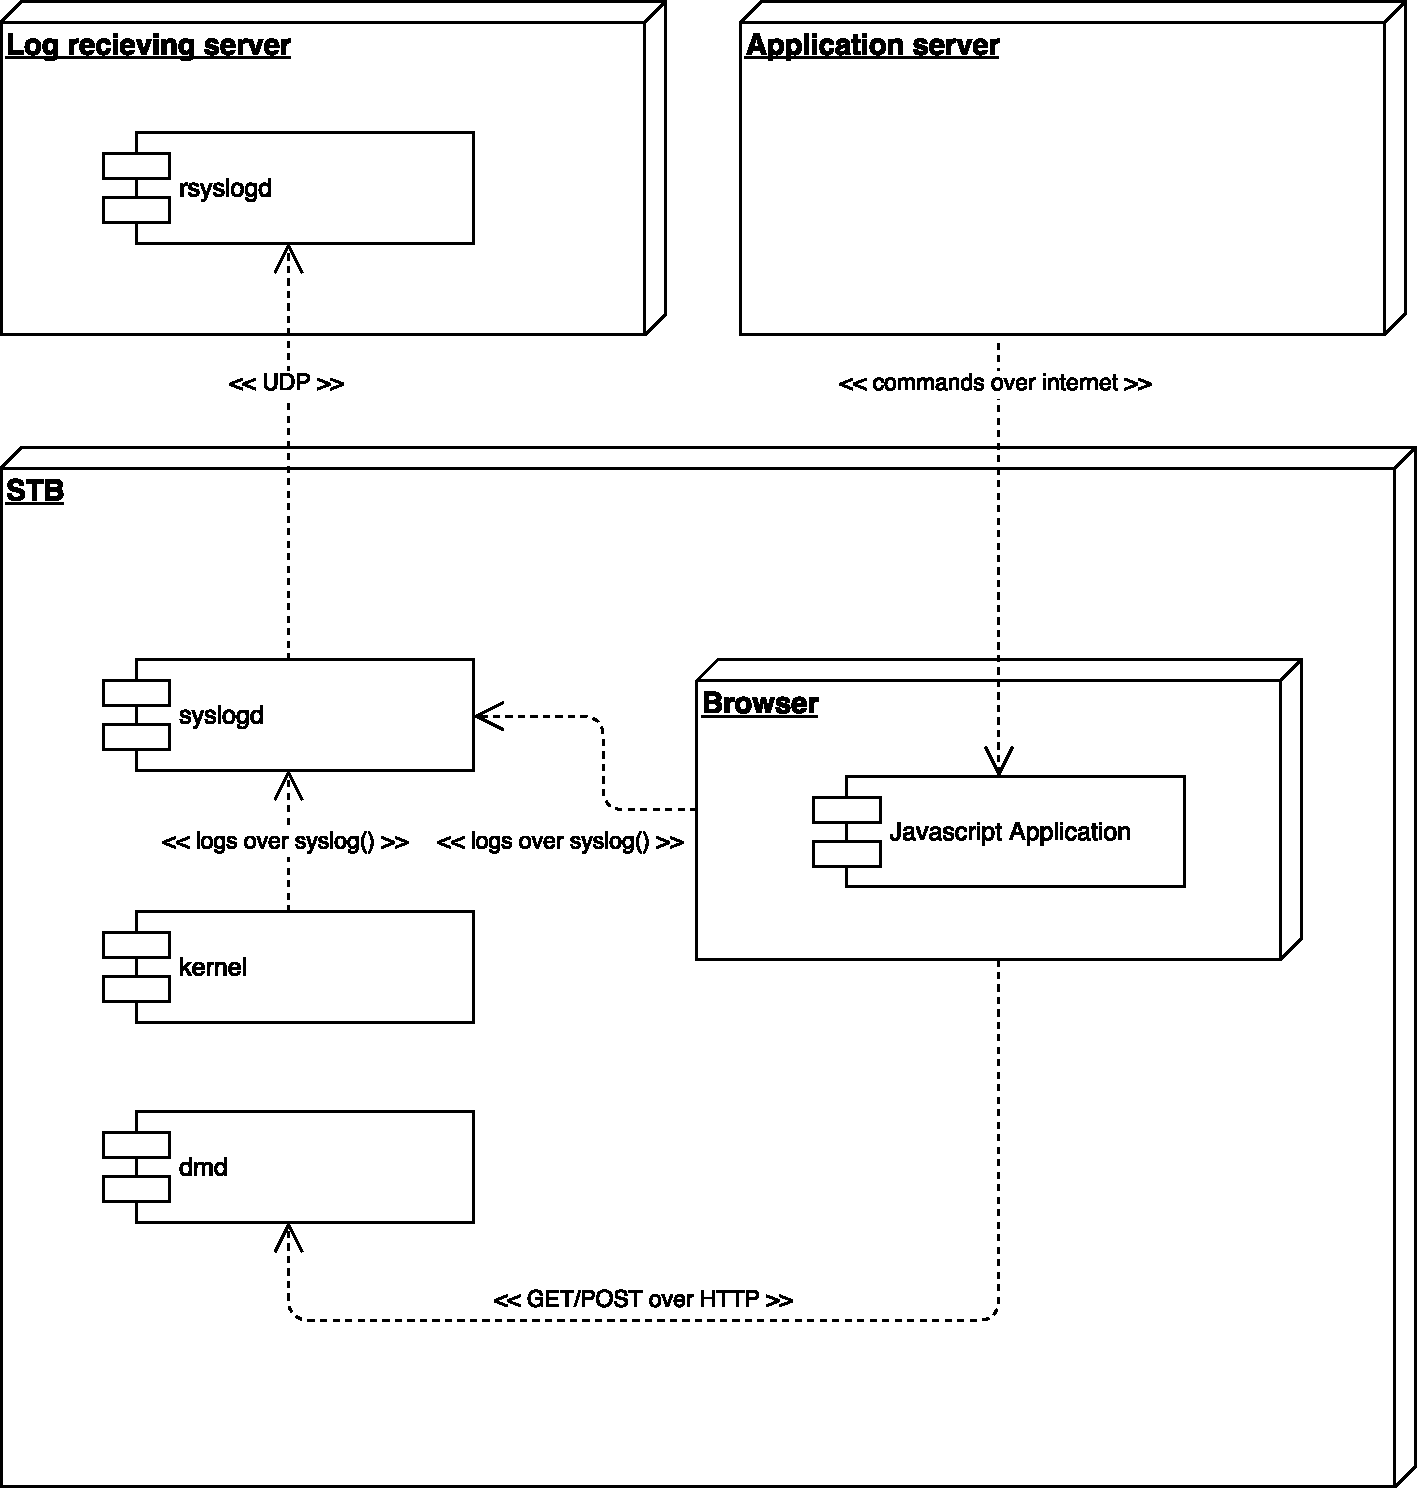
\includegraphics[scale=0.5]{images/STB}
	\caption[STB]{Diagram nasazení původního řešení STB}
\end{figure}

\section{Současné řešení}
V této kapitole jsou uvedeny a popsány jednotlivé pro tuto práci důlužité komponenty současného řešení.

\subsection{Runtime prostředí}
Na STB běží OS GNU/Linux s Busybox sadou aplikací, která nahrazuje standardní GNU shellové utility. Busybox aplikace jsou díky své malé velikosti vhodnější pro embedded zařízení. Na druhou stranu neobsahují všechny funkcionality a možnosti nastavení.

\subsubsection{Browser}
Browser je jednoduchý internetový prohlížeč dodaný výrobcem STB.
V něm běží v Javascriptu zadavatelem napsaná aplikace poskytující uživatelské rozhraní. Mimo to také naslouchá zprávám z aplikačního serveru, na jejichž základě může provádět akce, a to včetně generování POST či GET requestu pro démon dmd.
Tato javascriptová aplikace spolu s dalším podpogramem nesoucím název player generují velké množství logů. Tyto logy nepoužívají standardizovanou syslog množinu severit, ale svou vlastní s ní nekompatibilní. Logovací démon ovšem očekává zprávy právě podle syslog standardu. Implementaci browseru ani playeru nemůže zadavatel měnit a proto je třeba nekompatibilitu vyřešit pomocí logovacího démonu.

\subsubsection{Servisní komponenta dmd}
Dmd je v C++ napsaná servisní komponenta, která zprostředkovává komunikaci mezi Browserem a shellovým prostředím pomocí minimalistického HTTP serveru. Umožňuje JavaScript aplikaci na STB provádět operace, které jsou dostupné jen z shellového API.

\subsubsection{BusyBox Syslogd}
Jedná se o minimalistický logovací démon, který je podrobněji popsán v následující kapitole \uv{Srovnání logovacích démonů}.
Zadavatel mu pro své potřeby navíc doimplementoval číslování jednotlivých zpráv pro rozpoznání výpadku a za druhé naivní rate-limiting zpráv. Ten je naivní z důvodu, že používá statický buffer na počet zpráv, který nebere ohled na jejich velikost a hlavně bufferované zprávy se neodešlou samy, ale jen s nově příchozími zprávami.
Za použití tohoto démonu není možné splnit některé stěžejní technické požadavky, jako například \uv{Snížení objemu logů} nebo \uv{Post processing zpráv}. Proto bude nutné ho nahradit nějakým vyspělejším démonem. Tím se ale zabývá až další kapitola \uv{Nové řešení}.

\subsection{Aplikační server}
Aplikační server se stará o business logiku, například poskytuje uživateli práva přehrát daný kanál nebo film, komunikuje s javascriptovou aplikací, která se vůči němu autorizuje a podobně.
AS není možné v této práci jakkoli měnit. Je nutné zachovat kompatibilitu.

\subsection{Servery pro sběr logů}
Zadavatel provozuje cluster serverů sbírajících logy od statisíců STB. Běží na nich rsyslog nakonfigurovaný pro co nejlepší výkonost.


\section{Vývoj pro STB}
\subsection{Buildovací systém Gu}
Gu je buildovací systém pro linuxová embedded zařízení, který si klade za cíl zjednodušit a urychlit buildovací proces. Gu využívá balíčkovací systém pacman (převzatý z Arch Linuxu) a nástroj scratchbox2 sloužící k zjednodušení cross-kompilace. Tyto 2 nástroje jsou skryty v konzolovém přikazu \uv{gu}, kterým se celé Gu ovládá.

\subsection{PKGBUILD}
Jedná se o shellový script obsahující informace potřebné pro build jednotlivých aplikací systémem Gu. Níže je pro představu uveden vzorový script:
\begin{scriptsize}
\begin{verbatim}
pkgname=libee
pkgver=0.4.1
pkgrel=1
arch=('armv7h' 'armv7sp')
depends=('libestr')

build() {
    cd ${pkgname}-${pkgver}
    PKG_CONFIG_PATH=/mnt/hdd_1/lib/pkgconfig
    ./configure --prefix=/mnt/hdd_1
    make V=1
}

package() {
    cd ${pkgname}-${pkgver}
    make install DESTDIR=${pkgdir}
}
\end{verbatim}
\end{scriptsize}

Povinná pole jsou \uv{pkgname}, označující název balíčku, \uv{pkgver} pro určení jeho verze, \uv{pkgrel} sloužící k označení verze PKGBUILD scriptu a \uv{arch} definující cílové architektury.
 Script dále obsahuje funkce zajišťující build a instalaci balíčku. Každý PKGBUILD musí obsahovat minimálne funkci package(), která nainstaluje soubory do cílové složky. Užitečnou funkcí je funkce build() sloužící k přípravě a kompilaci zdrojových kódů před samotnou jejich instalací.

\section{Nové řešení}

\begin{figure}[!h]
	\centering
	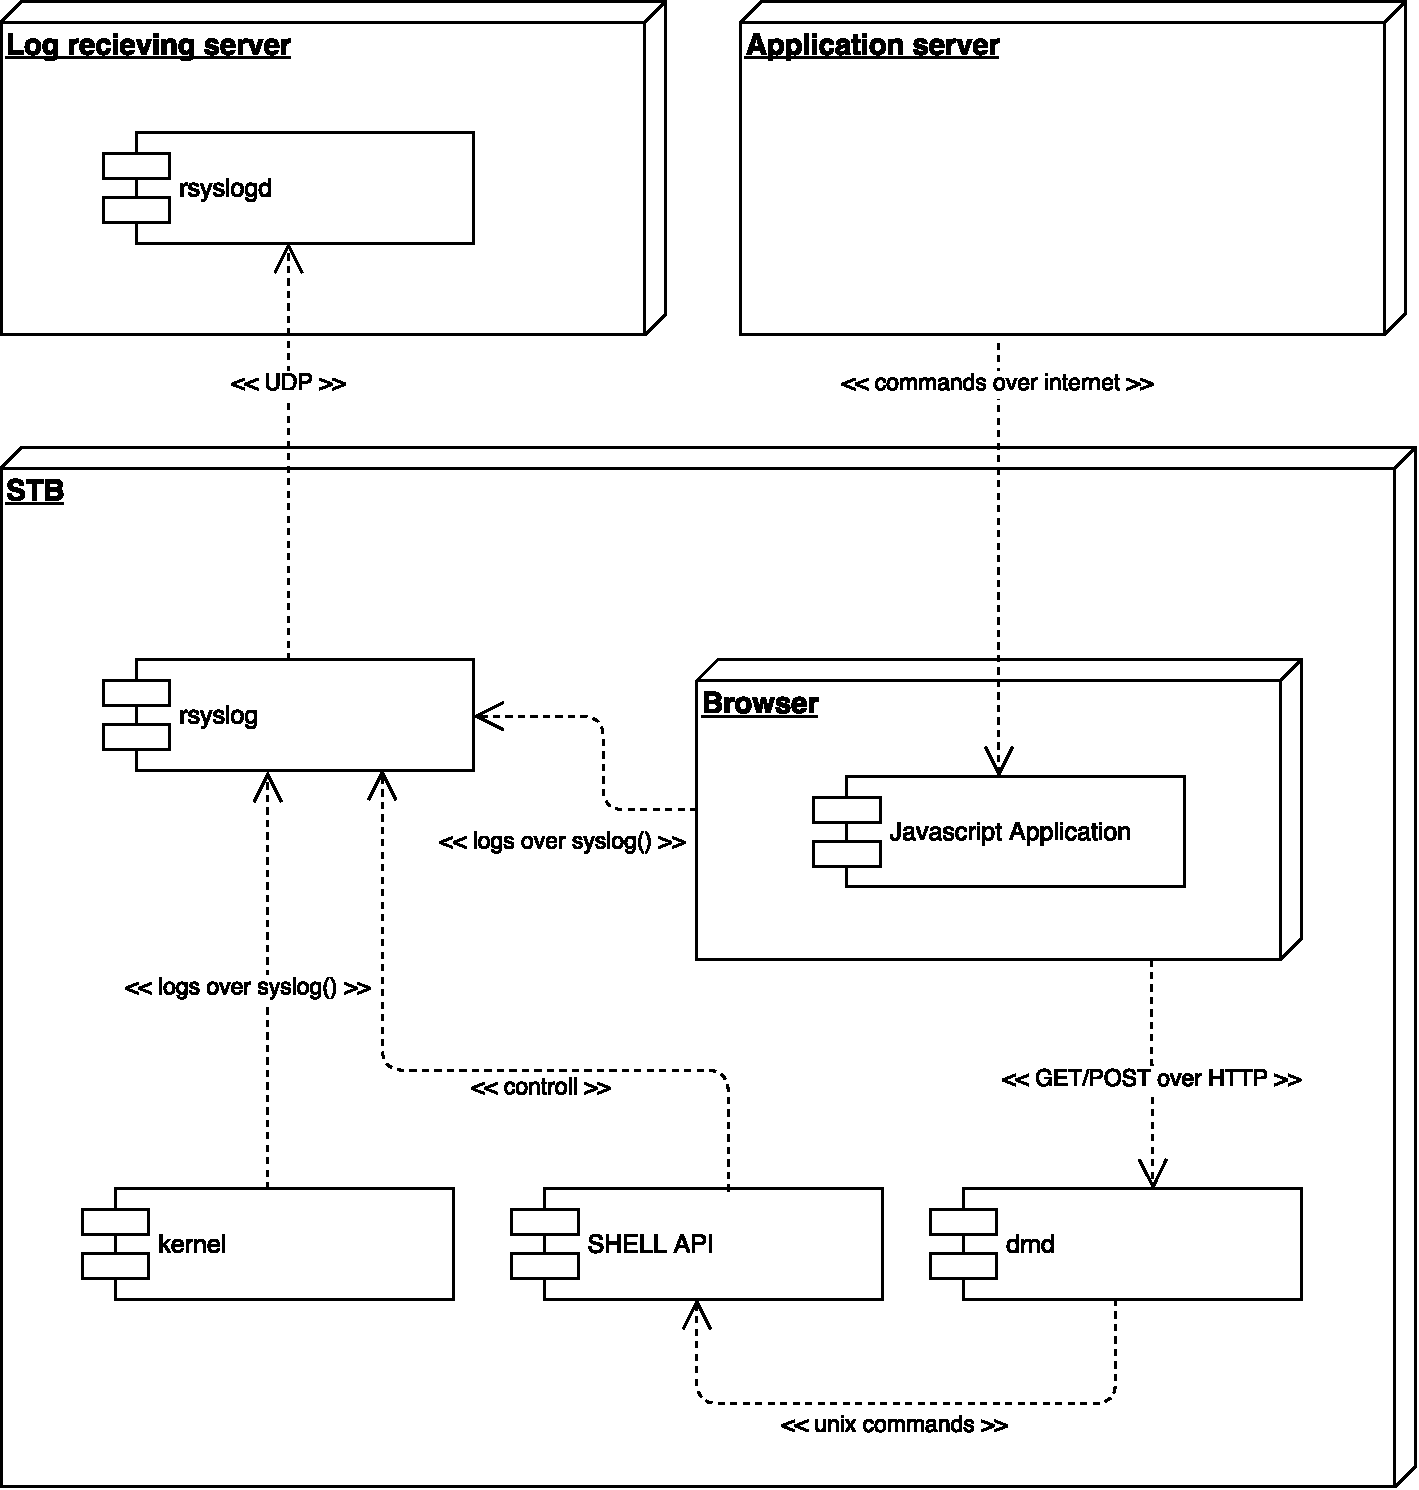
\includegraphics[scale=0.5]{images/STB-new}
	\caption[STB-new]{Diagram nasazení nového řešení STB}
\end{figure}

Prvně je nutno zvážit, zda problém řešit na straně serveru nebo set-top boxu. Vhodnou konfigurací logovacího démona na straně serveru, který by nepotřebné zprávy zavčas rozpoznal, zahodil a dále nezpracovával bychom splnili požadavek na snížení zátěže serverových disků. Přetížení sítě se takto vyřešit ale nedá a proto toto řešení zavrhuji.
Je tedy nutno problém řešit na straně set-top boxu kde původní řešení je postaveno na busy-box syslogd. Nabízí se možnost upravit fungování tím způsobem, aby se logy s nízkou severitou už na set-top boxu zahazovaly a pouze v případě potřeby bylo umožněné na dálku změnit konfiguraci démona tak, aby se povolilo logování pro logy s nastavenou danou komponentou a severitou. To vše přes SHELL-ové API.
Součástí zadání je ale i implementovat škrcení zpráv, aby nedocházelo k zahlcení linky. Takovou možnost prostý syslogd neposkytuje a je proto nutno zvážit napsání vlastního démona či nasazení jiného, vyspělejšího logovacího démona.


\section{Srovnání logovacích démonů}
Démon v UNIXovém světě je označení pro takový proces, který oproti běžným procesům neintereaguje přímo s uživatelem, ale běží na pozadí operačního systému a funguje samostatně. Účelem logovacího démona je sběr logů od ostatních procesů, které následně v závislosti na jeho konfiguraci dokáže filtrovat a ukládat na disk či odesílat na požadovaný vzdálený server.

V této kapitole zmíním a popíši vybrané logovací démony a v závěru kapitoly je porovnám.

\subsection*{BusyBox Syslogd}
Tato logovací utilita se skládá ze dvou démonů, jmenovitě z Klogd, který zachytává logy z kernelu a předává je ke zpracování Syslogdémonu. Syslogd pak zachytává i všechny zbylé logy a dále s nimi nakládá. Má však velice omezenou funkcionalitu. Dokáže pouze logy lokálně ukládat, přeposílat je dále po síti, zahazovat duplikáty, rotovat logy v závislosti na velikosti a filtrovat zprávy podle omezených kritérií. Dokáže totiž filtrovat pouze podle typu facility a už nikoliv podle názvu komponenty, která log vygenerovala.

\subsection*{Syslog-ng}
Flexibilní logovací démon zaměřený na centralizované a zabezpečené logování. Má široké možnosti nastavení a poskytuje obrovské množství funkcionalit. Takže jeho vhodným nakonfigurováním se dají snadno splnit všechny vytyčené technické požadavky až na požadavek pro možnost vzdálené změny konfigurace.
Je nutno ale zmínit, že pokročilé funkce jako například šifrování zpráv, bufferování nebo message-rate kontrola jsou dostupné pouze v komerční closed-source verzi.

\subsection*{Rsyslog}
Výčet funkcionalit Rsyslogu je ještě obsáhlejší než u Syslog-ng. Technické požadavky se s jeho použitím tedy také dají splnit všechny, kromě vzdálené změny konfigurace. Oproti Syslog-ng je Rsyslog kompletně zdarma a open-source. Navíc není jen logovacím démonem, ale i analyzérem logů. Dokáže logy podle obsahu zprávy měnit, třídit a jinak s nimy nakládat.
Že je Rsyslog vyspělý a kvalitní program dokazuje fakt, že je defaultním logovacím démonem na spoustě linuxových distribucích, jmenovitě například v Ubuntu.
Jeho slabiny shledávám v nedostatečné dokumentaci a ve specifických případech v neefektivním analyzování logů mající za následek (obvzláště na embedded zařízení s pomalým ARM procesorem) rychlostní deficit. Jeho vývoj obstarává z velké většiny pouze jeden člověk, jeho původní tvůrce Rainer Gerhards. A v jednom člověku není snadné dovést tak rozsáhlý projekt k dokonalosti.

\subsection*{Porovnání výše zmíněných logovacích utilit}
Pouhým nasazením jakéhokoli známého logovacího démonu není možné splnit všechny vytyčené technické požadavky. V případě ponechání původního BusyBox syslogd démonu by pro splnění technických požadavků bylo nutno doimplementovat tolik funkcionalit, že by to výrazně přesahovalo rozsah bakalářské práce.
Výhodněji se jeví nasadit pokročilý logovací démon jako je Syslog-ng či Rsyslog. Oba totiž poskytují námi požadované funkcionality. Syslog-ng však většinu z nich poskytuje pouze v placené closed-source verzi a proto jsem se rozhodl pro Rsyslog.

\section{Vzdálená konfigurace}
Rsyslog při svém zapnutí čte konfigurační soubor rsyslog.conf, který za jeho běhu není možné měnit. Je proto nutné napsat SHELL-ové API, které umožní na dálku přenastavit tento konfigurační soubor a restartovat Rsyslog. Rsyslog dokáže načíst nový konfigurační soubor zdánlivě i bez restartu a to po obdržení SIGHUP signálu. Avšak ve skutečnosti \cite{RsyslogHUP} k restartu dojde i tak a nelze se proto jeho restartování vyhnout.

Požadavkem zadavatele je umožnit změnu nastavení maximální povolené severity jednotlivých komponent. Tedy nastavit Rsyslog tak, aby v případě rozpoznání zprávy od určité komponenty spolu s nastavenou severitou vyšší, než je povolená, danou zprávu zahodil. Změny tímto skriptem způsobebé musí být zachovány i po restartu STB.

V této kapitole diskutuji možná řešení SHELLL-ového API. Samotná implementace je k nalezení v kapitole Realizace.

\subsection{Logika skriptu}
V úvahu připadaly 2 různé přístupy. Je možné při každém zavolání scriptu generovat celý nový konfigurační soubor a nebo parsovat stávající soubor a jeho část pomocí skriptu měnit.
Výhodou prvního způsobu je, že nehrozí nechtěné přepsání jiných čásí skriptu, než bylo zamýšleno. Nevýhodou je složitější implementace z důvodu nutnosti pří generování nového skriptu zohledňovat předchozí nastavení skritpu. Tedy by bylo nutno z původního skriptu extrahovat nastavení jednotlivých komponent a to zkombinovat s novým nastavením.
Rozhodl jsem se proto pro 2. způsob řešení s tím, že zadavatel bude poučen o nutnosti dodržovat určité zásady při měnění konfiguračního souboru, aby nemohlo dojít k neočekávanému chování.

\subsection{Rozhraní skriptu}
První možností je napsat API ve formě scriptu, který přijímá jednotlivé názvy komponent a jim příslušící maximální povolenou severitu jako parametry.
\begin{scriptsize}
\begin{verbatim}
set_log_verbosity.sh [component] [severity] [component2] [severity] ...
\end{verbatim}
\end{scriptsize}

Jako druhá možnost připadá v úvahu skript, který čte seznam jednotlivých komponent a maximálních povolených severit ze souboru, který má následující formát:

\begin{scriptsize}
\begin{verbatim}
/etc/logging.conf
\end{verbatim}}
\end{scriptsize}

\begin{scriptsize}
\begin{verbatim}
component1  = DEBUG
componentXY = INFO
...
DEFAULT     = INFO
\end{verbatim}
\end{scriptsize}

Se zadavatelem jsme se shodli, že se lépe jeví první způsob pro jeho jednoduší a rycheljší obsluhu a navíc s jeho použitím odpadá starost o další konfigurační soubor.

\section{Postprocessign zpráv}
Všechna níže zmíněná pravidla jsou myšlena jako vzory pro zadavatele, který podle nich v budoucnu vytvoří svá vlastní.
\subsection{Smazání podřetězce z těla syslog zprávy}
Zprávy s nastavenou severitou INFO a komponentou sld\_br je třeba změnit podle následujícího vzoru.

\subsubsection*{Originální zpráva:}
\begin{scriptsize}
\begin{verbatim}
2016-02-18T14:05:24+01:00 cc-b8-f1-00-6f-07 sld_br: id=559 
:[stbhal.cpp:debug:520]: INFO: [94mDEBUG: InformationService:
 Reading 'nangu.video.forcedScart': false[0m
\end{verbatim}}
\end{scriptsize}

\subsubsection*{Výsledná zpráva:}
\begin{scriptsize}
\begin{verbatim}
2016-02-18T14:05:24+01:00 cc-b8-f1-00-6f-07 sld_br: id=559
[94mDEBUG: InformationService: Reading 'nangu.video.forcedScart':
false[0m
\end{verbatim}}
\end{scriptsize}

\subsection{Zahazování zpráv podle typu komponenty}
Je třeba dokázat rozpoznat a zahodit zprávy podle zadané komponenty a obsahující určitý podřetězec.

\subsection{Převod severit}
Aplikace na STB používají pro logování jinou množinu severit, než s jakými pracuje Rsyslog. Zadavatel proto požaduje změnit severity zpráv podle následující tabulky.

\begin{table}[ht]
\centering
	\caption{Převodní tabulka}	\begin{tabular}{|l|l|}\hline
		Portal		& Syslog			\tabularnewline \hline \hline
		ERROR		& ERR			\tabularnewline \hline
		WARN		& WARN			\tabularnewline \hline
		INFO		& NOTICE			\tabularnewline \hline
		DEBUG		& INFO			\tabularnewline \hline
		TRACE		& DEBUG			\tabularnewline \hline
	\end{tabular}
\end{table}

\section{Rate-limiting zpráv}
Původní řešení obsahuje rate-limiting implementovaný tím způsobem, že do zdrojového kódu BusyBox syslogd, který je v jednom malém C souboru, byl doimplementován statický buffer s omezenou velikostí pro 128 kB zpráv.

V Rsyslogu se podobného efektu dá dosáhnout prostým nastavením modulu imuxsock, kde parametry RateLimit.Interval a RateLimit.Burst určují maximální povolený počet zpráv za daný počet sekund.
\begin{scriptsize}
\begin{verbatim}
module(load="imuxsock"             #Provides support for local system logging.
	SysSock.RateLimit.Interval="2" #Specifies the rate-limiting interval in seconds.
	SysSock.RateLimit.Burst="500"  #Specifies the rate-limiting burst in number of messages.
)
\end{verbatim}
\end{scriptsize}
Původní řešení trápí neduh, kdy k vyprázdnění bufferu dochází až s nově příchozí zprávou, což má za následek, že v případě zaplněného bufferu a následující delší odmlky nově příchozích zpráv může dojit k velkému zpoždení odeslání zpráv v ten moment uložených v bufferu. Tento problém se sofistikovanějišího Rsyslogu netýká.

V sekci Testování se zabývám hledáním ideálního nastavení těchto parametrů.

\chapter{Realizace}

\section{Rsyslog}

\subsection{build}
Rsyslog bylo nutno zkompilovat ze zdrojových kódů včetně mnoha závislostí.

\subsection{konfigurace}
TODO jednotlivy configurace pro pravidla, dodat ukázky configů..
krome popsani rsyslog.conf i logrotate etc all scripty
nebo mozna do jine podsekce toto
\subsection{modul mmstrdel}
\subsection{modul mmsevbalbab}


\section{Shell API}
Na STB je přítomna pouze minimalistická BusyBox implementace SHELLu nesoucí název ASH, která neposkytuje tak elegantní syntaxi a neposkytuje tolik rozšířených funkcionalit jako moderní SHELL-ové jazyky typu BASH. I přesto se s pomocí ASHe a základních UNIXových programů jako například GREP povedlo API naprogramovat.
Skript na vstupu očekává sudý počet parametrů, kde každý sudý parametr je název komponenty a liché parametry slouží pro definování severit.
Skript vyhledá v konfiguračním souboru rsyslog.conf řádek s danou komponentou a přenastaví maximální povolenou severitu. Skript kontrolojue správnost vstupních parametrů pro zabránení neočekávaného chování programu.
\begin{lstlisting}[language=Bash]
TODO code
\end{lstlisting}

\section{dmd}

\chapter{Testování}

\begin{conclusion}

\end{conclusion}

\bibliographystyle{csn690}
\bibliography{mybibliographyfile}

\appendix

\chapter{Seznam použitých zkratek}
% \printglossaries
\begin{description}
	\item[API] Application Programming Interface
	\item[ASH] Almquist Shell
	\item[dmd] Download manager daemon
	\item[STB] Set-top box
	\item[SIGHUP] Signal Hang Up
\end{description}

\chapter{Obsah přiloženého CD}

\begin{figure}
	\dirtree{%
		.1 readme.txt\DTcomment{stručný popis obsahu CD}.
		.1 exe\DTcomment{adresář se spustitelnou formou implementace}.
		.1 src.
		.2 impl\DTcomment{zdrojové kódy implementace}.
		.2 thesis\DTcomment{zdrojová forma práce ve formátu \LaTeX{}}.
		.1 text\DTcomment{text práce}.
		.2 thesis.pdf\DTcomment{text práce ve formátu PDF}.
		.2 BP\_Vavricka\_David\_2016.pdf\DTcomment{text práce ve formátu PDF}.
	}
\end{figure}

\end{document}
